\documentclass[10pt, aspectratio=169, handout]{beamer}
\usefonttheme{professionalfonts}

\mode<presentation>{
  \usetheme{Berkeley}
  \usecolortheme{beaver}
  \usefonttheme{default}
  \setbeamertemplate{navigation symbols}{}
  \setbeamertemplate{caption}[numbered]
}

\setbeamertemplate{footline}{%
  \leavevmode%
  \hbox{%
    \begin{beamercolorbox}[wd=.85\paperwidth,ht=2.5ex,dp=1ex,left]{author in head/foot}%
      \usebeamerfont{author in head/foot}Digital Signal Processing, Fall 2025%
    \end{beamercolorbox}%
    \begin{beamercolorbox}[wd=.15\paperwidth,ht=2.5ex,dp=1ex,right]{date in head/foot}%
      \hspace*{0.5em}\insertframenumber{} / \inserttotalframenumber\hspace*{0.5em}%
    \end{beamercolorbox}%
  }%
  \vskip0pt%
}

\usepackage[english]{babel}
\usepackage[utf8]{inputenc}
\usepackage{tikz}
\usepackage{pgfplots}
\usepgfplotslibrary{groupplots}
\usetikzlibrary{calc, positioning, arrows.meta, backgrounds, plotmarks, shapes.geometric}
\pgfplotsset{compat=newest}

\usepackage{array}
\usepackage{makecell}
\usepackage{verbatim}
\usepackage{graphicx}
\usepackage{amsfonts}
\usepackage{amsmath}
\usepackage{bm}
\usepackage{epstopdf}
\usepackage[absolute,overlay]{textpos}
\usepackage{hyperref}
\hypersetup{colorlinks=true, linkcolor=blue, urlcolor=cyan}

\title[DSP]{Discrete Time FIR Filtering}
\author{Maxx Seminario}
\institute{University of Nebraska-Lincoln}
\date{Fall 2025}

% Parameter definitions
\newcommand{\WpText}{0.4}
\newcommand{\WsText}{0.6}
\newcommand{\DeltaText}{0.01}
\newcommand{\LText}{7}

\pgfmathsetmacro{\wpval}{\WpText}
\pgfmathsetmacro{\wsval}{\WsText}
\pgfmathsetmacro{\deltaval}{\DeltaText}
\pgfmathsetmacro{\Lval}{\LText}

\begin{document}

%--------------------------------------------------
\begin{frame}
  \titlepage
\end{frame}



%--------------------------------------------------
\section{Introduction}

\begin{frame}{Introduction: FIR Filters in Digital Signal Processing}

\textbf{What are FIR Filters?}
\begin{itemize}
  \item \textbf{Finite Impulse Response (FIR):} Filter output depends only on current and past inputs
  \item Impulse response has \emph{finite} duration (eventually becomes zero)
  \item Fundamental building block in discrete-time signal processing
\end{itemize}

\vspace{0.3cm}
\textbf{General Form:}
\[
y[n] = \sum_{k=0}^{M} b_k x[n-k] = b_0 x[n] + b_1 x[n-1] + \cdots + b_M x[n-M]
\]

where $h[n] = b_n$ for $0 \leq n \leq M$ (impulse response coefficients)

\vspace{0.3cm}
\textbf{Key Advantages:}
\begin{itemize}
  \item \textbf{Always stable} (finite sum cannot diverge)
  \item \textbf{Exact linear phase possible} (symmetric delay, no distortion)
  \item \textbf{Simple structure} (no feedback, easy to implement)
\end{itemize}

\end{frame}


%--------------------------------------------------
\section{Implementation}

\begin{frame}{Discrete-Time Implementation of FIR Filters}

\begin{center}
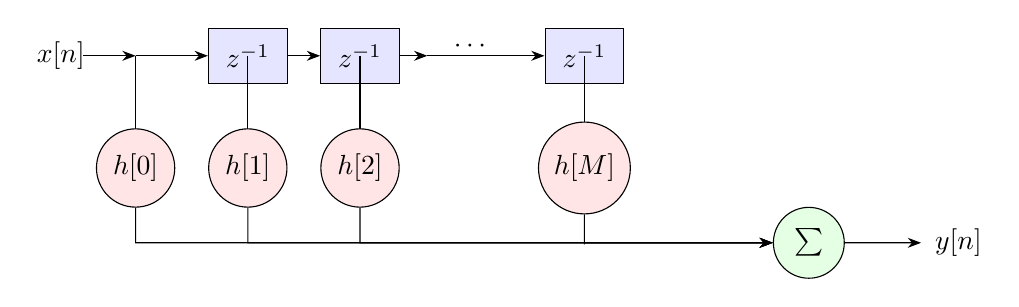
\begin{tikzpicture}[
  scale=0.95,
  delay/.style={rectangle, draw, minimum width=1.0cm, minimum height=0.7cm, fill=blue!10},
  mult/.style={circle, draw, minimum size=0.75cm, fill=red!10},
  sum/.style={circle, draw, minimum size=0.9cm, fill=green!10},
  >=Stealth
]

% Input
\node at (-1,0) {$x[n]$};
\draw[-{Stealth}] (-0.7,0) -- (0,0);

% Delay line (regular spacing)
\node[delay] (z1) at (1.5,0) {$z^{-1}$};
\node[delay] (z2) at (3.0,0) {$z^{-1}$};
\node at (4.5,0.12) {$\cdots$};          % place dots slightly above the line to avoid overlap
\node[delay] (zM) at (6.0,0) {$z^{-1}$};

% Multipliers (aligned with the taps)
\draw (0,0) -- (0,-1);
\node[mult] (h0) at (0,-1.5) {$h[0]$};

\draw (1.5,0) -- (1.5,-1);
\node[mult] (h1) at (1.5,-1.5) {$h[1]$};

\draw (3.0,0) -- (3.0,-1);
\node[mult] (h2) at (3.0,-1.5) {$h[2]$};

\draw (6.0,0) -- (6.0,-1);
\node[mult] (hM) at (6.0,-1.5) {$h[M]$};


\draw[-{Stealth}] (0,0) -- (z1);
\draw[-{Stealth}] (z1) -- (z2);
\draw[-{Stealth}] (z2) -- (3.9,0);         % stop short of the dots
\draw (3.9,0) -- (5.1,0);                  % short connector (no arrow) across the \cdots region
\draw[-{Stealth}] (5.1,0) -- (zM);

% Summer placed on same horizontal level as the multipliers' bottom horizontal lines
\node[sum] (sum) at (9.0,-2.5) {$\sum$};

\draw[-{Stealth}] (h0.south) -- ++(0,-0.4) -- (0,-2.5) -- (sum.west);
\draw[-{Stealth}] (h1.south) -- ++(0,-0.4) -- (1.5,-2.5) -- (sum.west);
\draw[-{Stealth}] (h2.south) -- ++(0,-0.4) -- (3.0,-2.5) -- (sum.west);
\draw[-{Stealth}] (hM.south) -- ++(0,-0.4) -- (6.0,-2.5) -- (sum.west);

% Output
\draw[-{Stealth}] (sum) -- (10.5,-2.5);
\node at (11.0,-2.5) {$y[n]$};

\end{tikzpicture}
\end{center}

% \vspace{0.2cm}
\textbf{Difference Equation:}
\[
y[n] = \sum_{k=0}^{M} h[k] \, x[n-k]
\]

\textbf{Computational Cost (per output sample):}
\begin{itemize}
  \item \textbf{Multiplications:} $M+1$
  \item \textbf{Additions:} $M$
  \item \textbf{Memory:} $M$ delay elements + $(M+1)$ coefficients
\end{itemize}

\end{frame}



%--------------------------------------------------
\section{Linear Phase FIR Filter Types}

\begin{frame}{Four Types of Linear-Phase FIR Filters}

\textbf{Classification by Symmetry and Length:}

\vspace{0.3cm}
\begin{center}
\begin{tabular}{|c|c|c|c|}
\hline
\textbf{Type} & \textbf{Length} & \textbf{Symmetry} & \textbf{Applications} \\
\hline
I & $(M+1)$ odd & Symmetric & Lowpass, highpass, bandpass \\
  & $M$ even & $h[n] = h[M-n]$ & Most versatile \\
\hline
II & $(M+1)$ even & Symmetric & Lowpass, bandpass \\
   & $M$ odd & $h[n] = h[M-n]$ & NOT for highpass \\
\hline
III & $(M+1)$ odd & Antisymmetric & Differentiators \\
    & $M$ even & $h[n] = -h[M-n]$ & Hilbert transformers \\
\hline
IV & $(M+1)$ even & Antisymmetric & Differentiators \\
   & $M$ odd & $h[n] = -h[M-n]$ & Hilbert transformers \\
\hline
\end{tabular}
\end{center}

\vspace{0.3cm}
\textbf{Key Distinction:}
\begin{itemize}
  \item \textbf{Symmetric} (Types I \& II): Real-valued frequency response
  \item \textbf{Antisymmetric} (Types III \& IV): Imaginary frequency response
\end{itemize}

\end{frame}

%--------------------------------------------------
\begin{frame}{Type I: Symmetric, Odd Length}

% \textbf{Properties:}
% \begin{itemize}
%   \item Filter length: $(M+1)$ with $M$ even
%   \item Symmetry: $h[n] = h[M-n]$ (symmetric about center)
%   \item Center sample: $h[M/2]$ can be non-zero
% \end{itemize}

% \vspace{0.2cm}
\textbf{Impulse Response Example ($M=8$, length = 9):}

\begin{center}
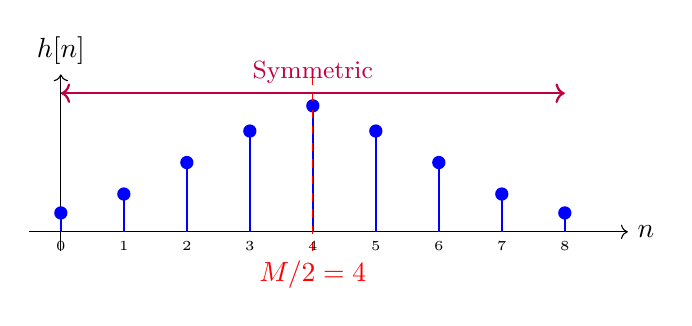
\begin{tikzpicture}[scale=0.8]
  \draw[->] (-0.5,0) -- (9,0) node[right] {$n$};
  \draw[->] (0,-0.3) -- (0,2. 5) node[above] {$h[n]$};
  
  % Symmetric impulse response
  \foreach \x/\h in {0/0.3, 1/0.6, 2/1.1, 3/1. 6, 4/2.0, 5/1.6, 6/1.1, 7/0.6, 8/0. 3} {
    \draw[thick, blue] (\x,0) -- (\x,\h);
    \fill[blue] (\x,\h) circle (3pt);
  }
  
  % Mark center
  \draw[dashed, red] (4,-0.3) -- (4,2.5);
  \node[below, red] at (4,-0.3) {$M/2=4$};
  
  % Show symmetry
  \draw[<->, thick, purple] (0,2.2) -- (8,2.2);
  \node[above, purple] at (4,2.2) {\small Symmetric};
  
  % Label samples
  \foreach \x in {0,1,2,3,4,5,6,7,8} {
    \node[below] at (\x,0) {\tiny $\x$};
  }
\end{tikzpicture}
\end{center}

\textbf{Frequency Response:}
\[
H(e^{j\omega}) = e^{-j\omega M/2} \underbrace{\left[ h[M/2] + 2\sum_{n=1}^{M/2} h[M/2-n]\cos(\omega n) \right]}_{\text{Real amplitude } A_e(e^{j\omega})}
\]

\end{frame}

%--------------------------------------------------
\begin{frame}{Type II: Symmetric, Even Length}

% \textbf{Properties:}
% \begin{itemize}
%   \item Filter length: $(M+1)$ with $M$ odd
%   \item Symmetry: $h[n] = h[M-n]$ (symmetric about center point between samples)
%   \item No center sample (center falls between two samples)
% \end{itemize}

% \vspace{0.2cm}
\textbf{Impulse Response Example ($M=7$, length = 8):}

\begin{center}
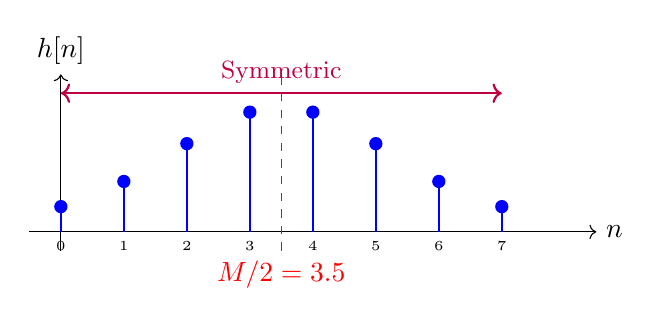
\begin{tikzpicture}[scale=0.8]
  \draw[->] (-0.5,0) -- (8. 5,0) node[right] {$n$};
  \draw[->] (0,-0.3) -- (0,2.5) node[above] {$h[n]$};
  
  % Symmetric impulse response
  \foreach \x/\h in {0/0. 4, 1/0.8, 2/1.4, 3/1.9, 4/1.9, 5/1.4, 6/0.8, 7/0. 4} {
    \draw[thick, blue] (\x,0) -- (\x,\h);
    \fill[blue] (\x,\h) circle (3pt);
  }
  
  % Mark center (between samples)
  \draw[dashed, red] (3.5,-0.3) -- (3.5,2.5);
  \node[below, red] at (3.5,-0.3) {$M/2=3. 5$};
  
  % Show symmetry
  \draw[<->, thick, purple] (0,2.2) -- (7,2.2);
  \node[above, purple] at (3.5,2.2) {\small Symmetric};
  
  % Label samples
  \foreach \x in {0,1,2,3,4,5,6,7} {
    \node[below] at (\x,0) {\tiny $\x$};
  }
\end{tikzpicture}
\end{center}

\textbf{Frequency Response:}
\[
H(e^{j\omega}) = e^{-j\omega M/2} \cos(\omega/2) \underbrace{P(\cos\omega)}_{\text{Polynomial}}
\]

\textbf{Limitation:} $\cos(\pi/2) = 0$ forces $H(e^{j\pi}) = 0$ (cannot realize highpass)

\end{frame}

%--------------------------------------------------

\begin{frame}{Efficient Implementation: Exploiting Symmetry}

\textbf{For Symmetric FIR Filters (Types I \& II):}

Since $h[n] = h[M-n]$, we can reduce computations by 50\% 

\begin{center}
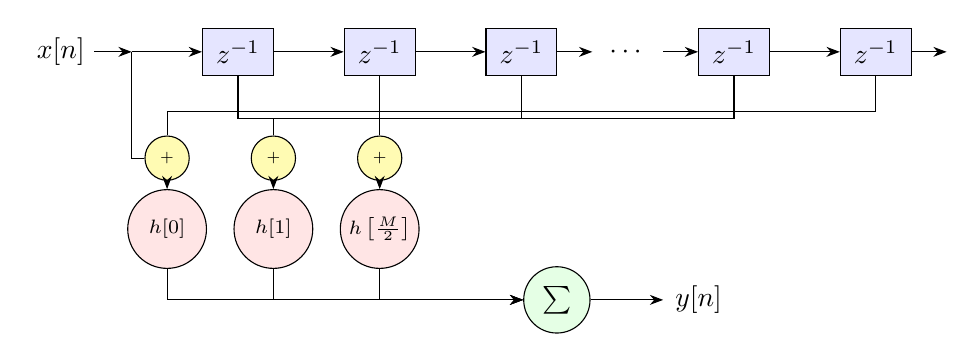
\begin{tikzpicture}[
  scale=0.9,
  >=Stealth,
  delay/.style={rectangle, draw, minimum width=0.9cm, minimum height=0.6cm, fill=blue!10},
  % make all multipliers the same fixed size (circle) so labels don't change shape
  mult/.style={circle, draw, minimum size=1.0cm, inner sep=0pt, align=center, fill=red!10},
  sum/.style={circle, draw, minimum size=0.8cm, fill=green!10},
  add/.style={circle, draw, minimum size=0.5cm, fill=yellow!30}
]

% Input
\node (xin) at (-1,0) {$x[n]$};
\draw[->] (xin) -- (0,0);

% Single delay line (left to right flow)
\node[delay] (z0) at (1.5,0) {$z^{-1}$};
\node[delay] (z1) at (3.5,0) {$z^{-1}$};
\node[delay] (z2) at (5.5,0) {$z^{-1}$};
\node at (7,0) {$\cdots$};
\node[delay] (z3) at (8.5,0) {$z^{-1}$};
\node[delay] (z4) at (10.5,0) {$z^{-1}$};

% Connect delays (straight line with dots)
\draw[->] (0,0) -- (z0);
\draw[->] (z0) -- (z1);
\draw[->] (z1) -- (z2);
\draw[->] (z2) -- ++(0.5,0) -- ++(0.5,0); % small gap to dots
\draw[->] (7.5,0) -- (z3);
\draw[->] (z3) -- (z4);
\draw[->] (z4) -- ++(1,0);

% Tap points for symmetric pairs (pre-adders)
% First pair: x[n] (input) and x[n-M] (at z4)
\node[add] (a0) at (0.5,-1.5) {\tiny $+$};
\draw (0,0) -- (0,-1) |- (a0);
\draw (z4.south) -- ++(0,-0.5) -| (a0);

% Second pair: x[n-1] (z0) and x[n-M+1] (z3)
\node[add] (a1) at (2,-1.5) {\tiny $+$};
\draw (z0.south) -- ++(0,-0.6) -| (a1);
\draw (z3.south) -- ++(0,-0.6) -| (a1);

% Third pair: x[n-2] (z1) and x[n-M+2] (z2)
\node[add] (a2) at (3.5,-1.5) {\tiny $+$};
\draw (z1.south) -- ++(0,-0.6) -| (a2);
\draw (z2.south) -- ++(0,-0.6) -| (a2);

% Multipliers - aligned on same y-level (-2.5)
% use \scriptsize inside nodes to keep labels compact but the circles identical in size
\node[mult] (m0) at (0.5,-2.5) {\scriptsize $h[0]$};
\draw[->] (a0) -- (m0);

\node[mult] (m1) at (2,-2.5) {\scriptsize $h[1]$};
\draw[->] (a1) -- (m1);

\node[mult] (m2) at (3.5,-2.5) {\scriptsize $h\left[\tfrac{M}{2}\right]$};
\draw[->] (a2) -- (m2);

% Final summation
\node[sum] (final) at (6,-3.5) {$\sum$};

% Direct arrows from each multiplier to final sum
% use |- so the path goes down first then right (vertical then horizontal)
\draw[->] (m0.south) |- (final.west);
\draw[->] (m1.south) |- (final.west);
\draw[->] (m2.south) |- (final.west);

% Output
\draw[->] (final) -- ++(1.5,0);
\node at (8,-3.5) {$y[n]$};

\end{tikzpicture}
\end{center}

\textbf{Optimized Cost: Trading Multiplies for Additions}
\begin{itemize}
  \item \textbf{Multiplications:} $\lceil (M+1)/2 \rceil$ (50\% reduction!)
  \item \textbf{Additions:} $M$ (pre-additions) + $\lceil (M+1)/2 \rceil - 1$ (post-additions)
  \item \textbf{Memory:} Still $M$ delays + $(M+1)$ coefficients
\end{itemize}

\end{frame}

%--------------------------------------------------
\begin{frame}{Type III: Antisymmetric, Odd Length}

% \textbf{Properties:}
% \begin{itemize}
%   \item Filter length: $(M+1)$ with $M$ even
%   \item Antisymmetry: $h[n] = -h[M-n]$ (antisymmetric about center)
%   \item Center sample: $h[M/2] = 0$ (forced by antisymmetry)
% \end{itemize}

% \vspace{0.2cm}
\textbf{Impulse Response Example ($M=8$, length = 9):}

\begin{center}
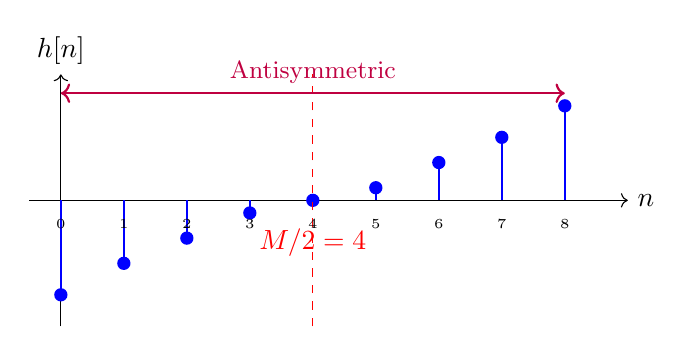
\begin{tikzpicture}[scale=0.8]
  \draw[->] (-0.5,0) -- (9,0) node[right] {$n$};
  \draw[->] (0,-2) -- (0,2) node[above] {$h[n]$};
  
  % Antisymmetric impulse response
  \foreach \x/\h in {0/-1.5, 1/-1.0, 2/-0.6, 3/-0.2, 4/0, 5/0.2, 6/0.6, 7/1.0, 8/1.5} {
    \draw[thick, blue] (\x,0) -- (\x,\h);
    \fill[blue] (\x,\h) circle (3pt);
  }
  
  % Mark center
  \draw[dashed, red] (4,-2) -- (4,2);
  \node[below, red] at (4,-0.3) {$M/2=4$};
  
  % Show antisymmetry
  \draw[<->, thick, purple] (0,1.7) -- (8,1.7);
  \node[above, purple] at (4,1. 7) {\small Antisymmetric};
  
  % Label samples
  \foreach \x in {0,1,2,3,4,5,6,7,8} {
    \node[below] at (\x,-0.15) {\tiny $\x$};
  }
\end{tikzpicture}
\end{center}

\textbf{Frequency Response:}
\[
H(e^{j\omega}) = j e^{-j\omega M/2} \sin(\omega) P(\cos\omega)
\]

% \textbf{Applications:} Differentiators ($\sin\omega \approx \omega$ for small $\omega$), Hilbert transformers
\textbf{Limitation:} $\sin(0) = 0$ forces $H(e^{j\pi0}) = 0$ (cannot realize lowpass)


\end{frame}

%--------------------------------------------------
\begin{frame}{Type IV: Antisymmetric, Even Length}

% \textbf{Properties:}
% \begin{itemize}
%   \item Filter length: $(M+1)$ with $M$ odd
%   \item Antisymmetry: $h[n] = -h[M-n]$ (antisymmetric about point between samples)
%   \item No center sample (center falls between two samples)
% \end{itemize}

% \vspace{0.2cm}
\textbf{Impulse Response Example ($M=7$, length = 8):}

\begin{center}
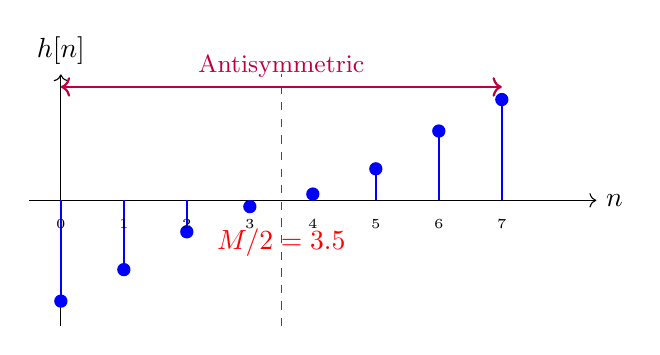
\begin{tikzpicture}[scale=0.8]
  \draw[->] (-0.5,0) -- (8.5,0) node[right] {$n$};
  \draw[->] (0,-2) -- (0,2) node[above] {$h[n]$};
  
  % Antisymmetric impulse response
  \foreach \x/\h in {0/-1.6, 1/-1.1, 2/-0.5, 3/-0.1, 4/0.1, 5/0.5, 6/1.1, 7/1. 6} {
    \draw[thick, blue] (\x,0) -- (\x,\h);
    \fill[blue] (\x,\h) circle (3pt);
  }
  
  % Mark center (between samples)
  \draw[dashed, red] (3. 5,-2) -- (3. 5,2);
  \node[below, red] at (3.5,-0.3) {$M/2=3.5$};
  
  % Show antisymmetry
  \draw[<->, thick, purple] (0,1.8) -- (7,1.8);
  \node[above, purple] at (3.5,1.8) {\small Antisymmetric};
  
  % Label samples
  \foreach \x in {0,1,2,3,4,5,6,7} {
    \node[below] at (\x,-0.15) {\tiny $\x$};
  }
\end{tikzpicture}
\end{center}

\textbf{Frequency Response:}
\[
H(e^{j\omega}) = j e^{-j\omega M/2} \sin(\omega/2) P(\cos\omega)
\]

% \textbf{Applications:} Differentiators, Hilbert transformers (most flexible antisymmetric type)
\textbf{Limitation:} $\sin(0) = 0$ forces $H(e^{j\pi(0)}) = 0$ (cannot realize lowpass)


\end{frame}

%--------------------------------------------------
\begin{frame}{Comparison: All Four Types}

\begin{center}
\scriptsize
\setlength{\tabcolsep}{6pt} % default is ~6pt
\renewcommand{\arraystretch}{1.0} %  row height
\begin{tabular}{|c|c|c|c|c|}
\hline
\textbf{Property} & \textbf{Type I} & \textbf{Type II} & \textbf{Type III} & \textbf{Type IV} \\
\hline
$M$ & Even & Odd & Even & Odd \\
\hline
Length $(M+1)$ & Odd & Even & Odd & Even \\
\hline
Symmetry & Sym & Sym & Antisym & Antisym \\
\hline
$h[M/2]$ & Non-zero & N/A & Zero & N/A \\
\hline
$H(0)$ & Any & Any & Zero & Non-zero \\
\hline
$H(\pi)$ & Any & Zero & Zero & Non-zero \\
\hline
\hline
Lowpass & \checkmark & \checkmark & $\times$ & $\times$ \\
\hline
Highpass & \checkmark & $\times$ & $\times$ & \checkmark \\
\hline
Bandpass & \checkmark & \checkmark & $\times$ & \checkmark \\
\hline
Differentiator & $\times$ & $\times$ & \checkmark & \checkmark \\
\hline
Hilbert & $\times$ & $\times$ & \checkmark & \checkmark \\
\hline
\end{tabular}
\end{center}

\vspace{0.2cm}
\textbf{Design Choice:}
\begin{itemize}
  \item Type I: Most versatile, use for general frequency-selective filters
  \item Type II: Lowpass only (response forced to zero at $\omega = \pi$)
  \item Types III \& IV: Specialized applications (differentiators, Hilbert)
\end{itemize}

\end{frame}

%--------------------------------------------------
\begin{frame}{Frequency Response Constraints}

\textbf{Why certain applications are prohibited:}

\vspace{0.3cm}
\begin{center}
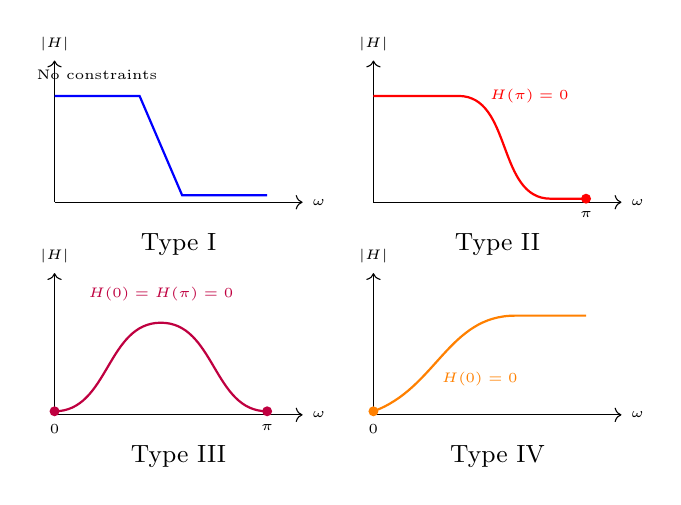
\begin{tikzpicture}[scale=0. 9]
  % Type I - no constraints
  \begin{scope}[xshift=0cm]
    \draw[->] (0,0) -- (3. 5,0) node[right] {\tiny $\omega$};
    \draw[->] (0,0) -- (0,2) node[above] {\tiny $|H|$};
    \draw[thick, blue] (0,1. 5) -- (1.2,1.5) -- (1.8,0.1) -- (3,0.1);
    \node[below] at (1.75,-0.3) {\small Type I};
    \node at (0.6,1.8) {\tiny No constraints};
  \end{scope}
  
  % Type II - zero at pi
  \begin{scope}[xshift=4. 5cm]
    \draw[->] (0,0) -- (3.5,0) node[right] {\tiny $\omega$};
    \draw[->] (0,0) -- (0,2) node[above] {\tiny $|H|$};
    \draw[thick, red] (0,1.5) -- (1.2,1. 5) to[out=0,in=180] (2.5,0.05) -- (3,0.05);
    \fill[red] (3,0.05) circle (2pt);
    \node[below] at (3,0) {\tiny $\pi$};
    \node[below] at (1.75,-0.3) {\small Type II};
    \node[red] at (2.2,1.5) {\tiny $H(\pi)=0$};
  \end{scope}
  
  % Type III - zero at 0 and pi
  \begin{scope}[xshift=0cm, yshift=-3cm]
    \draw[->] (0,0) -- (3.5,0) node[right] {\tiny $\omega$};
    \draw[->] (0,0) -- (0,2) node[above] {\tiny $|H|$};
    \draw[thick, purple] (0,0.05) to[out=0,in=180] (1.5,1.3) to[out=0,in=180] (3,0.05);
    \fill[purple] (0,0.05) circle (2pt);
    \fill[purple] (3,0.05) circle (2pt);
    \node[below] at (0,0) {\tiny $0$};
    \node[below] at (3,0) {\tiny $\pi$};
    \node[below] at (1.75,-0.3) {\small Type III};
    \node[purple] at (1.5,1.7) {\tiny $H(0)=H(\pi)=0$};
  \end{scope}
  
  % Type IV - zero at 0
  \begin{scope}[xshift=4.5cm, yshift=-3cm]
    \draw[->] (0,0) -- (3.5,0) node[right] {\tiny $\omega$};
    \draw[->] (0,0) -- (0,2) node[above] {\tiny $|H|$};
    \draw[thick, orange] (0,0.05) to[out=20,in=180] (2,1.4) -- (3,1.4);
    \fill[orange] (0,0.05) circle (2pt);
    \node[below] at (0,0) {\tiny $0$};
    \node[below] at (1.75,-0.3) {\small Type IV};
    \node[orange] at (1.5,0.5) {\tiny $H(0)=0$};
  \end{scope}
\end{tikzpicture}
\end{center}

\end{frame}



%--------------------------------------------------
\begin{frame}{FIR vs IIR Filters: Implementation Comparison}

\begin{center}
\small
\begin{tabular}{|p{3cm}|p{4cm}|p{4cm}|}
\hline
\textbf{Property} & \textbf{FIR Filters} & \textbf{IIR Filters} \\
\hline
\textbf{Stability} & 
\textcolor{green! 50! black}{\textbf{Always stable}} (no feedback) & 
\textcolor{red!70!black}{Can be unstable} (pole locations critical) \\
\hline
\textbf{Phase Response} & 
\textcolor{green!50!black}{\textbf{Exact linear phase}} possible (Types I-IV) & 
\textcolor{red!70!black}{Nonlinear phase} (except Bessel approximation) \\
\hline
\textbf{Filter Order} & 
\textcolor{red!70!black}{Higher order} needed (typically 10-100+ taps) & 
\textcolor{green!50!black}{\textbf{Lower order}} (typically 2-10 poles) \\
\hline
\textbf{Computation} & 
\textcolor{red!70!black}{More operations} per sample ($M+1$ multiplies) & 
\textcolor{green!50!black}{\textbf{Fewer operations}} (typically $< 10$ multiplies) \\
\hline
\textbf{Memory} & 
\textcolor{red!70!black}{More memory} ($M$ delays) & 
\textcolor{green!50!black}{\textbf{Less memory}} (order of filter) \\
\hline
\textbf{Finite Wordlength} & 
\textcolor{green!50! black}{\textbf{Robust}} (no limit cycles, low sensitivity) & 
\textcolor{red!70!black}{Sensitive} (limit cycles, pole location errors) \\
\hline
\textbf{Design} & 
\textcolor{green!50!black}{\textbf{Systematic}} (windowing, Parks-McClellan) & 
More complex (bilinear transform, pole placement) \\
\hline
\end{tabular}
\end{center}

\end{frame}

%--------------------------------------------------
\begin{frame}{When to Use FIR vs IIR Filters}

\begin{columns}

\column{0.48\textwidth}
\textbf{Choose FIR When:}
\begin{itemize}
  \item \textbf{Linear phase required}
  \begin{itemize}
    \item Audio processing
    \item Image processing
    \item Data transmission
  \end{itemize}
  
  \item \textbf{Stability critical}
  \begin{itemize}
    \item Safety systems
    \item Embedded systems
  \end{itemize}
  
  \item \textbf{Fixed-point implementation}
  \begin{itemize}
    \item Low wordlength DSPs
    \item Quantization robustness needed
  \end{itemize}
  
\end{itemize}

\column{0.48\textwidth}
\textbf{Choose IIR When:}
\begin{itemize}
  \item \textbf{Computational efficiency critical}
  \begin{itemize}
    \item Real-time constraints
    \item Low-power devices
    \item High sample rates
  \end{itemize}
  
  \item \textbf{Sharp transitions needed}
  \begin{itemize}
    \item Narrow stopband
    \item Steep rolloff
    \item Lower order achievable
  \end{itemize}
  
  \item \textbf{Memory limited}
  \begin{itemize}
    \item Small coefficient storage
    \item Few delay elements
  \end{itemize}
\end{itemize}

\end{columns}

\vspace{0.3cm}
\textbf{General rule of thumb:}
\begin{itemize}
  \item Use \textbf{FIR} for audio/video (linear phase) and when stability/robustness are critical
  \item Use \textbf{IIR} for control systems and when computational resources are constrained
\end{itemize}

\end{frame}






\end{document}